\documentclass[11pt,a4paper]{article}

\usepackage[utf8]{inputenc}
\usepackage{amsmath, amssymb, amsthm}
\usepackage{graphicx}
\usepackage{booktabs}
\usepackage{hyperref}
\usepackage[margin=2.5cm]{geometry}
\usepackage{tikz}
\usetikzlibrary{arrows.meta, positioning}
\usepackage{natbib}
\usepackage{xcolor}

\newcommand{\E}{\mathbb{E}}
\newcommand{\Var}{\mathrm{Var}}
\newcommand{\pa}{\mathrm{pa}}

\title{Causal Discovery via Pearson Risk Invariance:\\
Technical Report and Simulation Study}
\author{Technical report for the \texttt{causalreg} R package}
\date{\today}

\begin{document}
\maketitle

\begin{abstract}
This report describes the statistical method implemented in the \texttt{causalreg} R package for causal discovery in generalized linear models (GLMs) and generalized additive models (GAMs). The method exploits the fact that the Pearson risk equals~1 if and only if the model is correctly specified with respect to its causal parents. We present the theoretical foundations, describe the search algorithms, and evaluate the method's performance through a simulation study across five data-generating processes with varying sample sizes.
\end{abstract}

\tableofcontents

% ============================================================================
\section{Introduction}
% ============================================================================

Consider a structural causal model (SCM) where a target variable $Y$ is generated from its causal parents $\mathbf{X}_{\pa(Y)}$ through a generalized linear model or generalized additive model. Given a set of candidate covariates $\mathbf{X} = (X_1, \ldots, X_p)$ that includes both causal parents and non-causal variables (ancestors, descendants, confounders), the goal is to identify $\pa(Y) \subseteq \{1, \ldots, p\}$.

The \texttt{causalreg} package \citep{vinciotti2026} implements a method based on \emph{Pearson risk invariance}: the observation that the Pearson risk of a correctly specified GLM/GAM converges to~1, while misspecified models (wrong covariate set) yield a Pearson risk that deviates from~1.

% ============================================================================
\section{Methodology}
% ============================================================================

\subsection{Generalized Linear Models}

A GLM specifies the conditional distribution of $Y_i$ given covariates $\mathbf{x}_i$ through:
\begin{align}
Y_i &\sim \text{ExponentialFamily}(\mu_i, \phi), \\
g(\mu_i) &= \mathbf{x}_i^\top \boldsymbol{\beta},
\end{align}
where $g(\cdot)$ is the link function, $\mu_i = \E[Y_i \mid \mathbf{x}_i]$, and $\phi$ is the dispersion parameter. Common choices include:
\begin{itemize}
    \item \textbf{Poisson regression}: $Y_i \sim \text{Poisson}(\mu_i)$ with $g(\mu) = \log(\mu)$, so $\mu_i = \exp(\mathbf{x}_i^\top \boldsymbol{\beta})$.
    \item \textbf{Logistic regression}: $Y_i \sim \text{Bernoulli}(\mu_i)$ with $g(\mu) = \log(\mu/(1-\mu))$, so $\mu_i = \text{logistic}(\mathbf{x}_i^\top \boldsymbol{\beta})$.
\end{itemize}

\subsection{Generalized Additive Models}

A GAM extends the GLM by replacing the linear predictor with a sum of smooth functions:
\begin{equation}
g(\mu_i) = \beta_0 + \sum_{j=1}^{p} f_j(x_{ij}),
\end{equation}
where each $f_j$ is estimated nonparametrically (e.g., via penalized regression splines). This allows the method to discover causal relationships with nonlinear functional forms.

\subsection{Pearson Residuals and Pearson Risk}

For observation $i$ with fitted value $\hat{\mu}_i$ and variance function $V(\cdot)$, the \emph{Pearson residual} is:
\begin{equation}
r_i = \frac{Y_i - \hat{\mu}_i}{\sqrt{V(\hat{\mu}_i)}}.
\end{equation}

For Poisson models, $V(\mu) = \mu$, so $r_i = (Y_i - \hat{\mu}_i)/\sqrt{\hat{\mu}_i}$. For binomial models, $V(\mu) = \mu(1-\mu)$, so $r_i = (Y_i - \hat{\mu}_i)/\sqrt{\hat{\mu}_i(1-\hat{\mu}_i)}$.

The \emph{Pearson risk} is defined as:
\begin{equation}
\label{eq:pearson_risk}
R_P = \frac{1}{n} \sum_{i=1}^{n} r_i^2 = \frac{1}{n} \sum_{i=1}^{n} \frac{(Y_i - \hat{\mu}_i)^2}{V(\hat{\mu}_i)}.
\end{equation}

\subsection{The Invariance Principle}

The key theoretical result is:

\begin{quote}
\textbf{Pearson Risk Invariance.} If the model includes exactly the true causal parents of $Y$ (i.e., the covariates are $\mathbf{X}_{\pa(Y)}$), then $R_P \xrightarrow{p} 1$ as $n \to \infty$.

If the covariate set $S$ does not equal $\pa(Y)$---either by omitting a causal parent or including a non-causal variable that induces bias---then $R_P$ converges to a value different from~1.
\end{quote}

This provides a testable criterion for evaluating whether a candidate covariate set corresponds to the causal parents: test whether the Pearson risk equals~1.

\subsection{Hypothesis Testing}
\label{sec:testing}

Given a candidate covariate set $S$, we test:
\begin{equation}
H_0: R_P = 1 \quad \text{vs.} \quad H_1: R_P \neq 1.
\end{equation}

Two testing procedures are implemented:

\subsubsection{Chi-square test}

The Pearson statistic $X^2 = n \cdot R_P = \sum_{i=1}^n r_i^2$ follows approximately a $\chi^2_{n-p}$ distribution under $H_0$, where $p$ is the number of estimated parameters. The two-sided p-value is:
\begin{equation}
p_{\chi^2} = 2 \min\!\big(P(\chi^2_{n-p} \leq X^2),\; P(\chi^2_{n-p} \geq X^2)\big).
\end{equation}
This approximation is valid for Poisson models but not reliable for binomial models.

\subsubsection{Bootstrap test}

For general families (including binomial), a nonparametric bootstrap test is used:
\begin{enumerate}
    \item For $b = 1, \ldots, B$:
    \begin{enumerate}
        \item Draw a bootstrap sample $\{(Y_i^{*}, \mathbf{x}_i^{*})\}_{i=1}^n$ by sampling with replacement.
        \item Fit the model to the bootstrap sample to obtain $\hat{\mu}_i^{*(b)}$.
        \item Compute the bootstrap Pearson risk: $R_P^{(b)} = \frac{1}{n}\sum_{i=1}^n \frac{(Y_i^{*} - \hat{\mu}_i^{*(b)})^2}{V(\hat{\mu}_i^{*(b)})}$.
    \end{enumerate}
    \item Compute $\hat{p} = \frac{1}{B}\sum_{b=1}^B \mathbf{1}(R_P^{(b)} \geq 1)$.
    \item The p-value is $p_{\text{boot}} = 2 \min(\hat{p},\; 1 - \hat{p})$.
\end{enumerate}

The default number of bootstrap replicates is $B = 100$.

\subsection{Model Selection}

A covariate set $S$ is \emph{causally valid} if its Pearson risk p-value exceeds the significance level~$\alpha$ (default $\alpha = 0.05$). Among all causally valid sets, the one with the lowest BIC is selected:
\begin{equation}
\hat{S} = \arg\min_{S:\; p_S > \alpha} \text{BIC}(S).
\end{equation}

The BIC criterion serves as a parsimony tie-breaker: if multiple covariate sets pass the Pearson risk test, the most parsimonious well-fitting model is preferred.

\subsection{Search Strategies}
\label{sec:search}

\subsubsection{Exhaustive search (\texttt{search = "all"})}

All $2^p - 1$ non-empty subsets of the $p$ covariates are evaluated. For each subset, the model is fitted, the Pearson risk p-value is computed, and the BIC is recorded. The subset with the lowest BIC among those passing the test is returned.

This guarantees finding the global optimum but has exponential complexity: it becomes impractical for $p > 15$.

\subsubsection{Stepwise search (\texttt{search = "stepwise"})}

A two-phase greedy search:

\paragraph{Forward phase.} Starting from the intercept-only model, at each step:
\begin{enumerate}
    \item For each remaining candidate variable, fit the model with that variable added and compute the Pearson risk p-value.
    \item Select the variable whose addition yields the highest p-value.
    \item Continue if the p-value increased compared to the previous step, or if it exceeds $\alpha$.
\end{enumerate}

\paragraph{Backward BIC phase.} Starting from the model obtained by the forward phase:
\begin{enumerate}
    \item For each variable currently in the model, compute the BIC of the model without that variable.
    \item If removing a variable improves BIC, remove it and repeat.
    \item Stop when no removal improves BIC.
\end{enumerate}

The stepwise search has $O(p^2)$ complexity per phase, making it feasible for large~$p$.

\subsection{Handling Categorical Variables in Binomial Models}

For binomial family models, an additional post-processing step handles categorical covariates. If the selected model contains categorical variables, the method tests whether removing them (individually or collectively) still yields a causally valid model. This addresses the fact that categorical variables can create spurious associations in logistic regression.

% ============================================================================
\section{Simulation Study}
% ============================================================================

\subsection{Data Generating Processes}

We evaluate the method on five data-generating processes (DGPs) taken from the package examples. Each DGP defines a structural causal model with known causal parents of~$Y$.

\subsubsection{DGP~1: Poisson GLM, $p = 2$}

\begin{center}
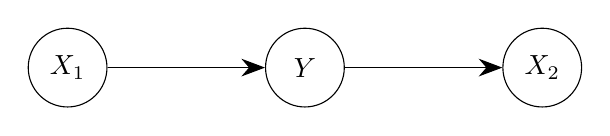
\begin{tikzpicture}[>={Stealth[length=3mm]}, node distance=2cm, every node/.style={draw, circle, minimum size=1cm}]
    \node (X1) {$X_1$};
    \node (Y)  [right=of X1] {$Y$};
    \node (X2) [right=of Y]  {$X_2$};
    \draw[->] (X1) -- (Y);
    \draw[->] (Y) -- (X2);
\end{tikzpicture}
\end{center}

\begin{align}
X_1 &\sim \mathcal{N}(0, 1), \\
Y \mid X_1 &\sim \text{Poisson}(\exp(X_1)), \\
X_2 &= \log(Y + 1) + \varepsilon, \quad \varepsilon \sim \mathcal{N}(0, 0.3^2).
\end{align}

True causal parents: $\pa(Y) = \{X_1\}$. The variable $X_2$ is a noisy downstream effect of $Y$.

\subsubsection{DGP~2: Binomial GLM, $p = 2$}

\begin{center}
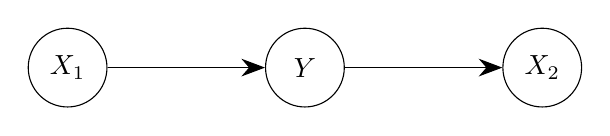
\begin{tikzpicture}[>={Stealth[length=3mm]}, node distance=2cm, every node/.style={draw, circle, minimum size=1cm}]
    \node (X1) {$X_1$};
    \node (Y)  [right=of X1] {$Y$};
    \node (X2) [right=of Y]  {$X_2$};
    \draw[->] (X1) -- (Y);
    \draw[->] (Y) -- (X2);
\end{tikzpicture}
\end{center}

\begin{align}
X_1 &\sim \mathcal{N}(0, 1), \\
Y \mid X_1 &\sim \text{Bernoulli}\!\left(\frac{\exp(X_1)}{1 + \exp(X_1)}\right), \\
X_2 &= (1 - F) \cdot Y + \varepsilon, \quad F \sim \text{Bernoulli}(0.1),\; \varepsilon \sim \mathcal{N}(0, 0.3^2).
\end{align}

True causal parents: $\pa(Y) = \{X_1\}$. The variable $X_2$ is a noisy copy of $Y$ with random label flipping.

\subsubsection{DGP~3: Binomial GLM, $p = 5$}

\begin{center}
\begin{tikzpicture}[>={Stealth[length=3mm]}, node distance=1.8cm, every node/.style={draw, circle, minimum size=1cm}]
    \node (X1) {$X_1$};
    \node (X2) [right=of X1] {$X_2$};
    \node (Y)  [right=of X2] {$Y$};
    \node (X3) [above=1.2cm of Y] {$X_3$};
    \node (X4) [below=1.2cm of X2] {$X_4$};
    \node (X5) [right=of Y] {$X_5$};
    \draw[->] (X1) -- (X2);
    \draw[->] (X2) -- (Y);
    \draw[->] (X3) -- (Y);
    \draw[->] (X2) -- (X4);
    \draw[->] (Y) -- (X5);
\end{tikzpicture}
\end{center}

\begin{align}
X_1 &\sim \mathcal{N}(0, 1), \quad X_2 \sim \mathcal{N}(X_1, 0.5^2), \quad X_3 \sim \mathcal{N}(0, 1), \\
X_4 &\sim \mathcal{N}(X_2, 0.5^2), \\
Y \mid X_2, X_3 &\sim \text{Bernoulli}\!\left(\frac{\exp(0.8 X_2 - 0.9 X_3)}{1 + \exp(0.8 X_2 - 0.9 X_3)}\right), \\
X_5 &= (1-F) \cdot Y + F \cdot (1-Y) + \varepsilon, \quad F \sim \text{Bernoulli}(0.1).
\end{align}

True causal parents: $\pa(Y) = \{X_2, X_3\}$. The challenges are: $X_1$ is an ancestor (correlated with $X_2$), $X_4$ is a descendant of $X_2$, and $X_5$ is a noisy descendant of $Y$.

\subsubsection{DGP~4: Poisson GAM, $p = 2$}

Same DAG structure as DGP~1, but with a nonlinear causal mechanism:
\begin{align}
X_1 &\sim \mathcal{N}(0, 1), \\
Y \mid X_1 &\sim \text{Poisson}(\exp(\sin(X_1))), \\
X_2 &= \log(Y + 1) + \varepsilon, \quad \varepsilon \sim \mathcal{N}(0, 0.5^2).
\end{align}

True causal parents: $\pa(Y) = \{X_1\}$ via the smooth function $s(X_1)$.

\subsubsection{DGP~5: Poisson GAM, $p = 7$}

A complex structural causal model with seven covariates and nonlinear relationships:
\begin{align}
X_1 &\sim \mathcal{N}(0, 0.04), \quad X_2 = X_1 + \varepsilon_2, \quad X_3 = X_1 + X_2 + \varepsilon_3, \\
m &= \sin(5 X_2) + X_3^3, \quad Z = m + \varepsilon_Z, \\
X_4 &= X_2 + \varepsilon_4, \quad X_5 = Z + \varepsilon_5, \quad X_6 = Z + \varepsilon_6, \quad X_7 = X_6 + \varepsilon_7, \\
Y &= Q_{\text{Pois}}\!\big(\Phi(Z; m, 0.04),\; \lambda = \exp(m)\big),
\end{align}
where all $\varepsilon_j \sim \mathcal{N}(0, 0.04)$, $\Phi$ is the normal CDF, and $Q_{\text{Pois}}$ is the Poisson quantile function.

True causal parents: $\pa(Y) = \{X_2, X_3\}$ via smooth functions $s(X_2)$ and $s(X_3)$.

\subsection{Experimental Setup}

For each DGP, we vary the sample size $n$ and the method configuration:

\begin{itemize}
    \item \textbf{Sample sizes}: $n \in \{200, 500, 1000, 2000, 3000\}$ (DGP-dependent).
    \item \textbf{Search strategies}: exhaustive (\texttt{all}) and stepwise (\texttt{stepwise}).
    \item \textbf{P-value methods}: chi-square and bootstrap ($B = 100$), where applicable.
    \item \textbf{Significance level}: $\alpha = 0.05$.
    \item \textbf{Replicates}: 100 independent datasets per scenario.
\end{itemize}

The bootstrap p-value method is used for binomial models (DGPs~2--3), as the chi-square approximation is unreliable. Both methods are compared for Poisson models (DGP~1).

For DGP~5 ($p = 7$), only the stepwise search is evaluated, as the exhaustive search over $2^7 - 1 = 127$ GAM models is computationally prohibitive for a simulation study.

\subsection{Metrics}

\begin{itemize}
    \item \textbf{Exact recovery rate}: fraction of replicates where the selected model contains exactly the true causal parents (no more, no less).
    \item \textbf{True positive rate (TPR)}: average fraction of true parents included in the selected model.
    \item \textbf{Average false positives}: average number of non-parent variables included.
\end{itemize}

% ============================================================================
\section{Results}
% ============================================================================

\subsection{Summary Table}

Table~\ref{tab:results} reports the exact recovery rate, true positive rate, and average number of false positives across all scenarios.

\begin{table}[htbp]
\centering
\caption{Simulation results: exact recovery rate, true positive rate, and average false positives across 100 replicates per scenario.}
\label{tab:results}
\small
\begin{tabular}{llrrrrr}
\toprule
DGP & Method & $n$ & Recovery & TPR & Avg.\ FP & Avg.\ found \\
\midrule
Poisson GLM (p=2) & all + chi-sq & 200 & 95\% & 0.95 & 0.00 & 0.9 \\
Poisson GLM (p=2) & all + chi-sq & 500 & 96\% & 0.96 & 0.00 & 1.0 \\
Poisson GLM (p=2) & all + chi-sq & 1000 & 88\% & 0.88 & 0.00 & 0.9 \\
Poisson GLM (p=2) & all + chi-sq & 2000 & 91\% & 0.91 & 0.00 & 0.9 \\
Poisson GLM (p=2) & step + chi-sq & 200 & 100\% & 1.00 & 0.00 & 1.0 \\
Poisson GLM (p=2) & step + chi-sq & 500 & 100\% & 1.00 & 0.00 & 1.0 \\
Poisson GLM (p=2) & step + chi-sq & 1000 & 100\% & 1.00 & 0.00 & 1.0 \\
Poisson GLM (p=2) & step + chi-sq & 2000 & 100\% & 1.00 & 0.00 & 1.0 \\
Poisson GLM (p=2) & all + boot & 200 & 90\% & 0.90 & 0.00 & 0.9 \\
Poisson GLM (p=2) & all + boot & 500 & 89\% & 0.89 & 0.00 & 0.9 \\
Poisson GLM (p=2) & all + boot & 1000 & 94\% & 0.94 & 0.00 & 0.9 \\
Poisson GLM (p=2) & all + boot & 2000 & 96\% & 0.96 & 0.00 & 1.0 \\
Poisson GLM (p=2) & step + boot & 200 & 95\% & 0.95 & 0.00 & 0.9 \\
Poisson GLM (p=2) & step + boot & 500 & 93\% & 0.93 & 0.00 & 0.9 \\
Poisson GLM (p=2) & step + boot & 1000 & 97\% & 0.97 & 0.00 & 1.0 \\
Poisson GLM (p=2) & step + boot & 2000 & 99\% & 0.99 & 0.00 & 1.0 \\
\midrule
Binomial GLM (p=2) & all + boot & 500 & 13\% & 0.97 & 0.86 & 1.8 \\
Binomial GLM (p=2) & all + boot & 1000 & 45\% & 0.95 & 0.50 & 1.4 \\
Binomial GLM (p=2) & all + boot & 2000 & 79\% & 0.94 & 0.15 & 1.1 \\
Binomial GLM (p=2) & step + boot & 500 & 19\% & 0.96 & 0.80 & 1.8 \\
Binomial GLM (p=2) & step + boot & 1000 & 42\% & 0.99 & 0.57 & 1.6 \\
Binomial GLM (p=2) & step + boot & 2000 & 78\% & 0.93 & 0.15 & 1.1 \\
\midrule
Binomial GLM (p=5) & all + boot & 1000 & 15\% & 0.93 & 1.11 & 3.0 \\
Binomial GLM (p=5) & all + boot & 2000 & 48\% & 0.98 & 0.69 & 2.7 \\
Binomial GLM (p=5) & all + boot & 3000 & 67\% & 0.97 & 0.48 & 2.4 \\
Binomial GLM (p=5) & step + boot & 1000 & 35\% & 0.94 & 0.62 & 2.5 \\
Binomial GLM (p=5) & step + boot & 2000 & 53\% & 0.96 & 0.44 & 2.4 \\
Binomial GLM (p=5) & step + boot & 3000 & 80\% & 0.94 & 0.15 & 2.0 \\
\midrule
Poisson GAM (p=2) & all + chi-sq & 500 & 92\% & 0.92 & 0.03 & 0.9 \\
Poisson GAM (p=2) & all + chi-sq & 1000 & 96\% & 0.96 & 0.00 & 1.0 \\
Poisson GAM (p=2) & all + chi-sq & 2000 & 95\% & 0.95 & 0.00 & 0.9 \\
Poisson GAM (p=2) & step + chi-sq & 500 & 100\% & 1.00 & 0.00 & 1.0 \\
Poisson GAM (p=2) & step + chi-sq & 1000 & 100\% & 1.00 & 0.00 & 1.0 \\
Poisson GAM (p=2) & step + chi-sq & 2000 & 100\% & 1.00 & 0.00 & 1.0 \\
\midrule
Poisson GAM (p=7) & step + chi-sq & 500 & 62\% & 0.67 & 0.37 & 1.7 \\
Poisson GAM (p=7) & step + chi-sq & 1000 & 64\% & 0.69 & 0.35 & 1.7 \\
\bottomrule
\end{tabular}

\end{table}

\subsection{Recovery Rate by Sample Size}

Figure~\ref{fig:recovery} shows the exact recovery rate as a function of sample size for each DGP.

\begin{figure}[htbp]
\centering
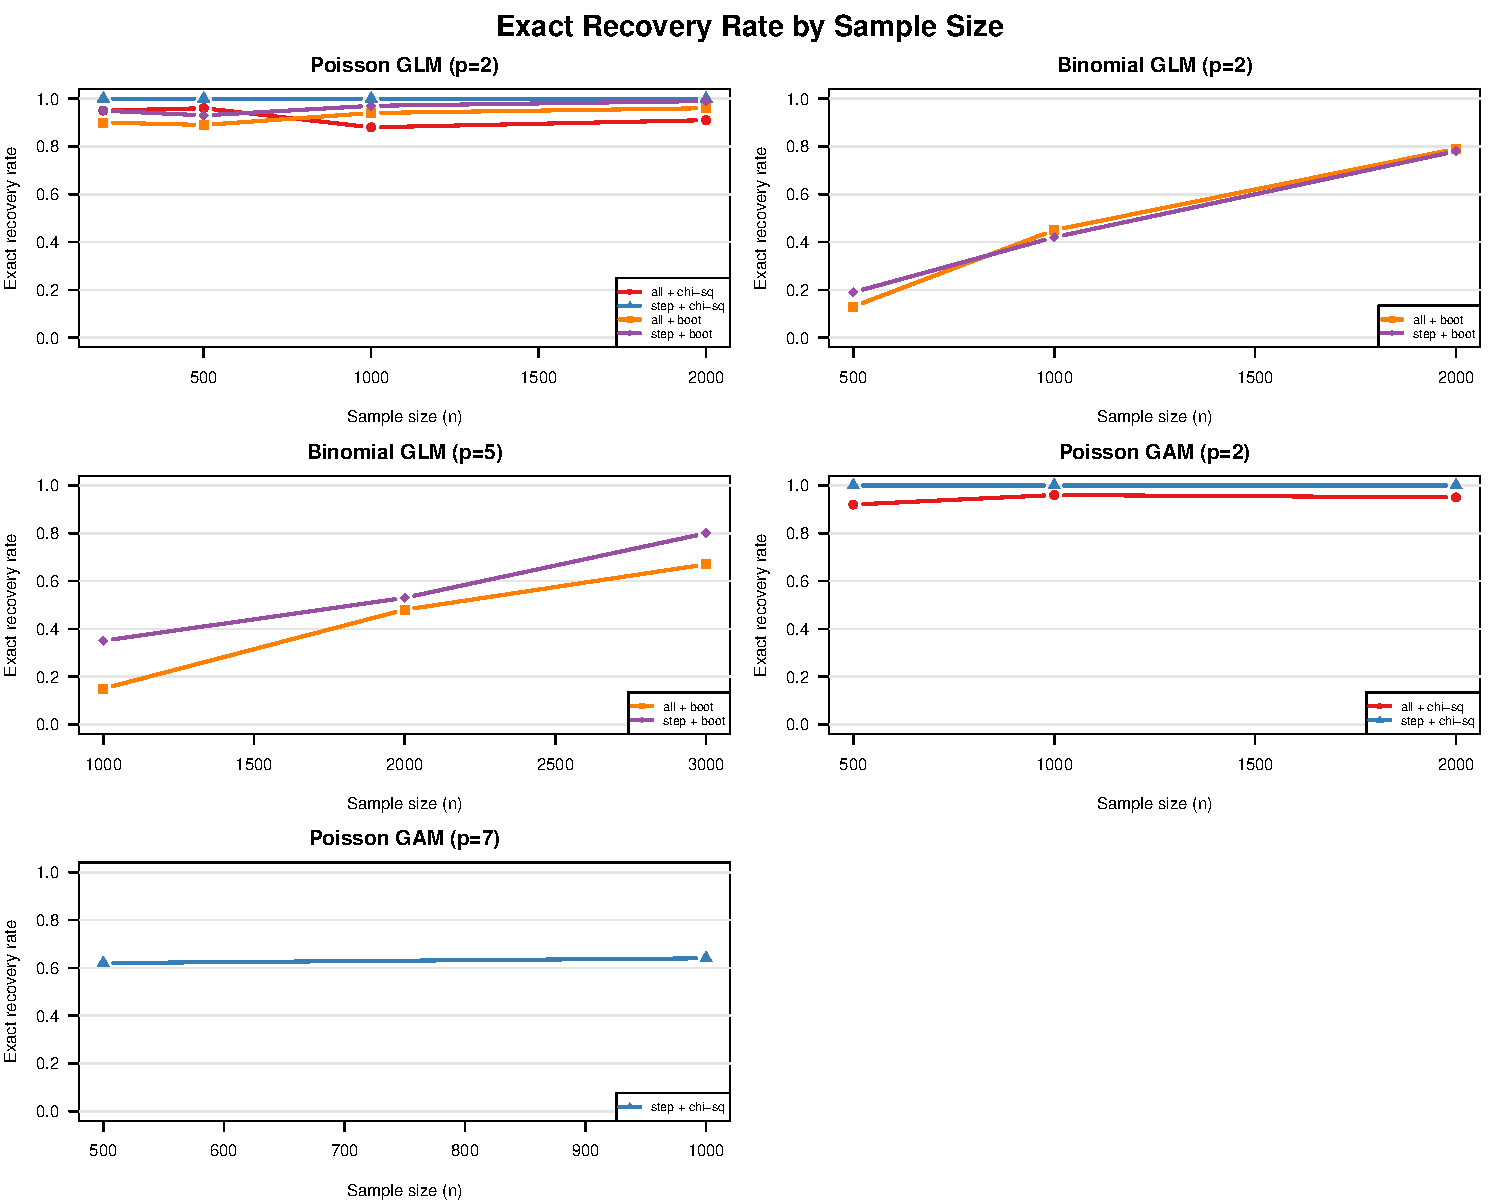
\includegraphics[width=\textwidth]{figures/fig_recovery_by_n.pdf}
\caption{Exact recovery rate by sample size for each data-generating process. Different line styles correspond to different method configurations (search strategy and p-value method).}
\label{fig:recovery}
\end{figure}

\subsection{Chi-square vs.\ Bootstrap P-value}

Figure~\ref{fig:chisq_boot} compares the chi-square and bootstrap p-value methods for the Poisson GLM (DGP~1). Both methods are applicable here, allowing a direct comparison.

\begin{figure}[htbp]
\centering
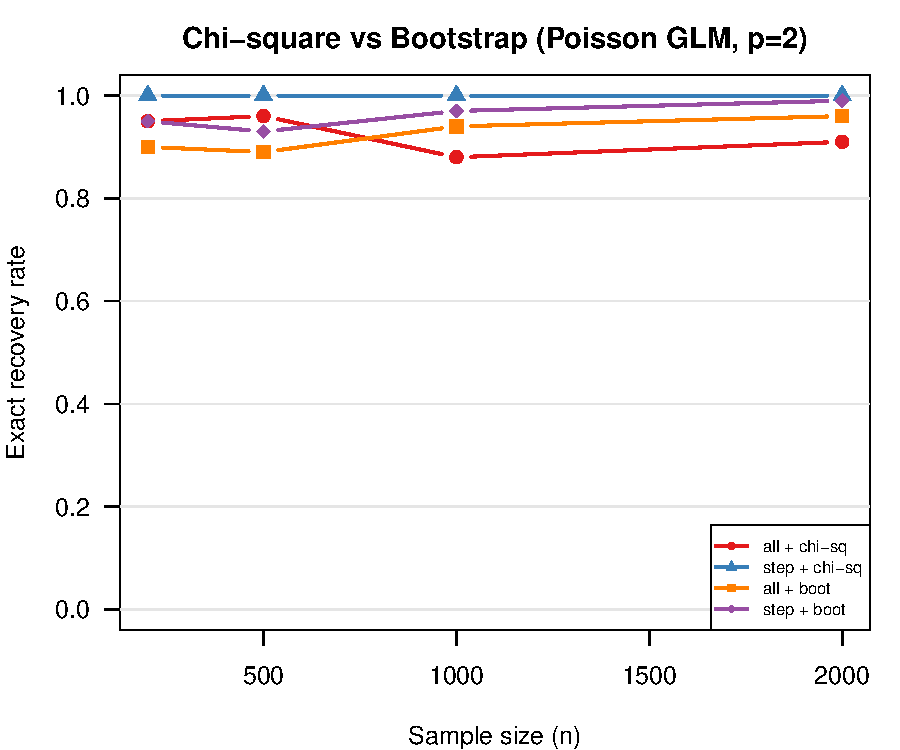
\includegraphics[width=0.65\textwidth]{figures/fig_chisq_vs_bootstrap.pdf}
\caption{Comparison of chi-square and bootstrap p-value methods for Poisson GLM with $p=2$ covariates.}
\label{fig:chisq_boot}
\end{figure}

\subsection{Detailed Analysis: Five-Covariate Binomial Case}

Figure~\ref{fig:p5detail} provides a detailed view of the five-covariate binomial case (DGP~3), which is the most challenging linear scenario.

\begin{figure}[htbp]
\centering
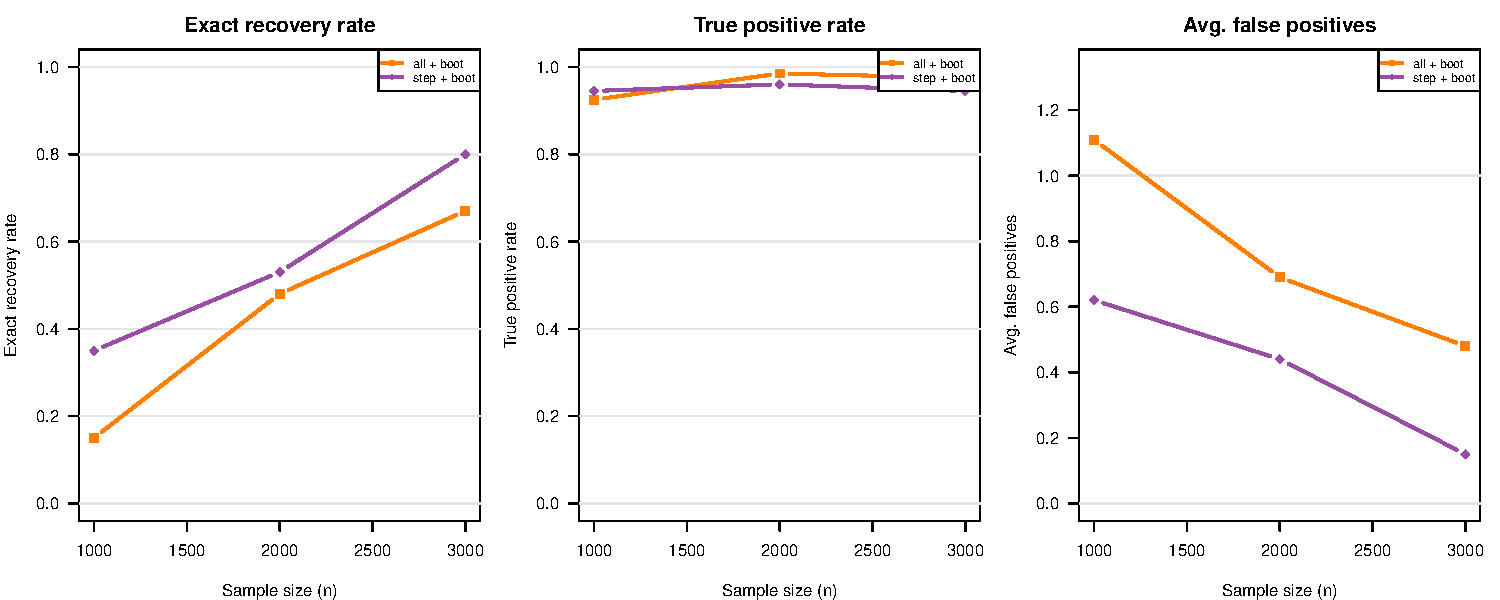
\includegraphics[width=\textwidth]{figures/fig_binomial_p5_detail.pdf}
\caption{Detailed metrics for the binomial GLM with $p=5$ covariates: exact recovery rate, true positive rate, and average false positives.}
\label{fig:p5detail}
\end{figure}

% ============================================================================
\section{Comparison with Adversarial Causal Regularization}
% ============================================================================

We now compare the Pearson risk invariance method (\texttt{causalreg}) with Adversarial Causal Regularization (ACR) \citep{richter2026}, a fundamentally different approach to causal discovery.

\subsection{ACR Method Overview}

ACR discovers causal relationships by exploiting the \emph{invariance principle}: the conditional distribution $P(Y \mid \mathbf{X}_{\pa(Y)})$ is invariant across environments, while spurious correlations change. Unlike \texttt{causalreg}, ACR does not require knowledge of the response family (Poisson, binomial); instead, it learns \emph{latent environment memberships} from data.

\paragraph{Phase~1: Adversarial weight learning.} ACR introduces soft weights $w_i \in [0,1]$ for each observation, partitioning the data into two pseudo-environments. The adversary maximizes the weighted risk difference (WRD):
\begin{equation}
\mathcal{L}(\boldsymbol{\beta}, \mathbf{w}) = \hat{R}_1(\boldsymbol{\beta}; \mathbf{w}) + \hat{R}_2(\boldsymbol{\beta}; \mathbf{w}) + \Gamma \cdot \big|\hat{R}_1(\boldsymbol{\beta}; \mathbf{w}) - \hat{R}_2(\boldsymbol{\beta}; \mathbf{w})\big|,
\end{equation}
where $\hat{R}_k$ are weighted mean squared errors for each pseudo-environment, and $\Gamma$ controls the adversarial strength.

The learner simultaneously updates $\boldsymbol{\beta}$ via a closed-form weighted ridge regression (Eq.~14 in \citealt{richter2026}):
\begin{equation}
\boldsymbol{\beta} = (\mathbf{G}_+ + \Gamma s \mathbf{G}_\Delta + \lambda \mathbf{I})^{-1}(\mathbf{Z}_+ + \Gamma s \mathbf{Z}_\Delta),
\end{equation}
where $s = \text{sgn}(\hat{R}_1 - \hat{R}_2)$, $\mathbf{G}_+, \mathbf{G}_\Delta$ are sums and differences of weighted Gram matrices, and $\lambda$ is a ridge penalty.

\paragraph{Phase~2: Cross-validated $\Gamma$ selection.} The regularization strength $\Gamma_{\text{fit}}$ is selected via $K$-fold cross-validation using the WRD criterion. The final coefficients are re-estimated with the selected $\Gamma_{\text{fit}}$.

\paragraph{Variable selection from ACR.} ACR produces a coefficient vector $\hat{\boldsymbol{\beta}}$. We select variable $j$ as a causal parent if $|\hat{\beta}_j| / \max_k |\hat{\beta}_k| > 0.15$ (relative magnitude threshold).

\subsection{Key Differences}

\begin{center}
\begin{tabular}{lll}
\toprule
& \textbf{causalreg} & \textbf{ACR} \\
\midrule
Input data & Single environment & Multi-env.\ (or discovers latent envs.) \\
Response type & Poisson, Binomial (GLM/GAM) & Continuous (MSE loss) \\
Output & Selected parent set & Coefficient vector \\
Variable selection & Via Pearson risk test + BIC & Via coefficient thresholding \\
Environment info & Not needed & Discovered from data \\
Nonlinear effects & Via GAM smooth terms & Not supported (linear) \\
\bottomrule
\end{tabular}
\end{center}

\subsection{Comparison Setup}

To compare the methods, we create multi-environment versions of DGPs~1--3 by introducing distribution shifts in downstream (non-causal) variables between environments. The data from both environments is pooled:

\begin{itemize}
    \item \textbf{causalreg} receives the pooled data and applies its Pearson risk invariance test, ignoring the environment structure.
    \item \textbf{ACR} receives the pooled data (without environment labels) and attempts to discover the latent environments via adversarial weight learning, then uses them for invariance-based variable selection.
\end{itemize}

Note that ACR uses MSE loss even on Poisson/Binomial responses, which is suboptimal but allows direct comparison. We also test ACR on a Gaussian linear DGP (its native setting) as a reference.

\subsection{Comparison Results}

Table~\ref{tab:comparison} and Figure~\ref{fig:comparison} show the comparison results.

\begin{table}[htbp]
\centering
\caption{Comparison of causalreg and ACR: exact recovery rate, true positive rate, average false positives, and computation time (per run) across 100 replicates.}
\label{tab:comparison}
\small
\begin{tabular}{llrrrrr}
\toprule
DGP & Method & $n$ & Recovery & TPR & Avg.\ FP & Time (s) \\
\midrule
Poisson GLM (p=2) & causalreg (all) & 500 & 96\% & 0.98 & 0.02 & 0.01 \\
Poisson GLM (p=2) & causalreg (step) & 500 & 98\% & 1.00 & 0.02 & 0.01 \\
Poisson GLM (p=2) & ACR & 500 & 0\% & 1.00 & 1.00 & 0.19 \\
Poisson GLM (p=2) & causalreg (all) & 1000 & 100\% & 1.00 & 0.00 & 0.01 \\
Poisson GLM (p=2) & causalreg (step) & 1000 & 100\% & 1.00 & 0.00 & 0.02 \\
Poisson GLM (p=2) & ACR & 1000 & 1\% & 1.00 & 0.99 & 0.23 \\
Poisson GLM (p=2) & causalreg (all) & 2000 & 100\% & 1.00 & 0.00 & 0.02 \\
Poisson GLM (p=2) & causalreg (step) & 2000 & 100\% & 1.00 & 0.00 & 0.04 \\
Poisson GLM (p=2) & ACR & 2000 & 0\% & 1.00 & 1.00 & 0.34 \\
\midrule
Binomial GLM (p=2) & causalreg (all) & 500 & 1\% & 0.08 & 0.99 & 0.66 \\
Binomial GLM (p=2) & causalreg (step) & 500 & 91\% & 1.00 & 0.09 & 0.65 \\
Binomial GLM (p=2) & ACR & 500 & 0\% & 0.99 & 1.00 & 0.17 \\
Binomial GLM (p=2) & causalreg (all) & 1000 & 91\% & 0.99 & 0.09 & 1.25 \\
Binomial GLM (p=2) & causalreg (step) & 1000 & 91\% & 0.98 & 0.08 & 1.25 \\
Binomial GLM (p=2) & ACR & 1000 & 0\% & 0.99 & 1.00 & 0.30 \\
Binomial GLM (p=2) & causalreg (all) & 2000 & 2\% & 1.00 & 0.98 & 2.18 \\
Binomial GLM (p=2) & causalreg (step) & 2000 & 3\% & 0.99 & 0.96 & 2.14 \\
Binomial GLM (p=2) & ACR & 2000 & 0\% & 1.00 & 1.00 & 0.50 \\
\midrule
Binomial GLM (p=5) & causalreg (all) & 1000 & 0\% & 0.99 & 1.99 & 12.21 \\
Binomial GLM (p=5) & causalreg (step) & 1000 & 1\% & 1.00 & 1.97 & 5.65 \\
Binomial GLM (p=5) & ACR & 1000 & 0\% & 0.99 & 2.00 & 0.35 \\
Binomial GLM (p=5) & causalreg (all) & 2000 & 0\% & 0.99 & 2.92 & 20.28 \\
Binomial GLM (p=5) & causalreg (step) & 2000 & 1\% & 0.99 & 1.97 & 9.79 \\
Binomial GLM (p=5) & ACR & 2000 & 0\% & 0.99 & 2.00 & 0.60 \\
Binomial GLM (p=5) & causalreg (all) & 3000 & 0\% & 0.98 & 2.04 & 31.42 \\
Binomial GLM (p=5) & causalreg (step) & 3000 & 2\% & 0.99 & 1.94 & 14.52 \\
Binomial GLM (p=5) & ACR & 3000 & 0\% & 1.00 & 2.00 & 0.89 \\
\midrule
Gaussian linear (p=5) & ACR & 500 & 0\% & 1.00 & 2.00 & 0.31 \\
Gaussian linear (p=5) & ACR & 1000 & 0\% & 1.00 & 2.00 & 0.39 \\
Gaussian linear (p=5) & ACR & 2000 & 0\% & 1.00 & 2.00 & 0.58 \\
\bottomrule
\end{tabular}

\end{table}

\begin{figure}[htbp]
\centering
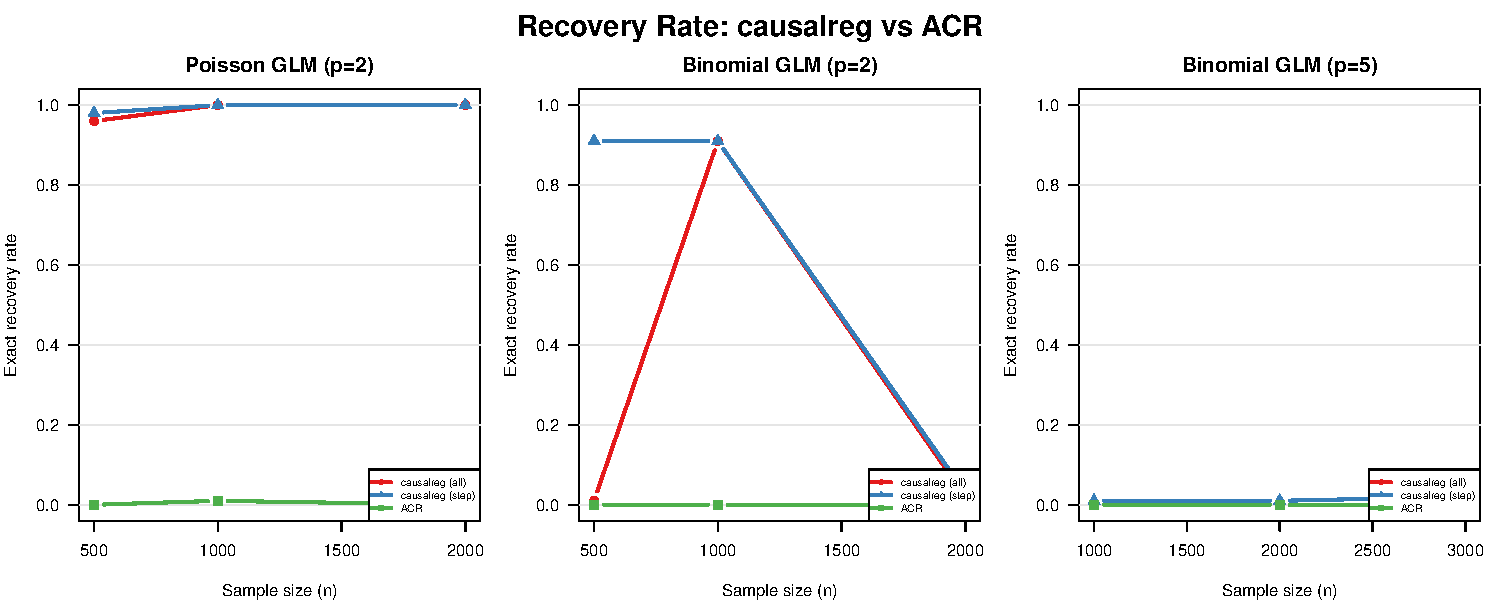
\includegraphics[width=\textwidth]{figures/fig_comparison_recovery.pdf}
\caption{Exact recovery rate comparison between \texttt{causalreg} (exhaustive and stepwise search) and ACR across three DGPs with varying sample size.}
\label{fig:comparison}
\end{figure}

\begin{figure}[htbp]
\centering
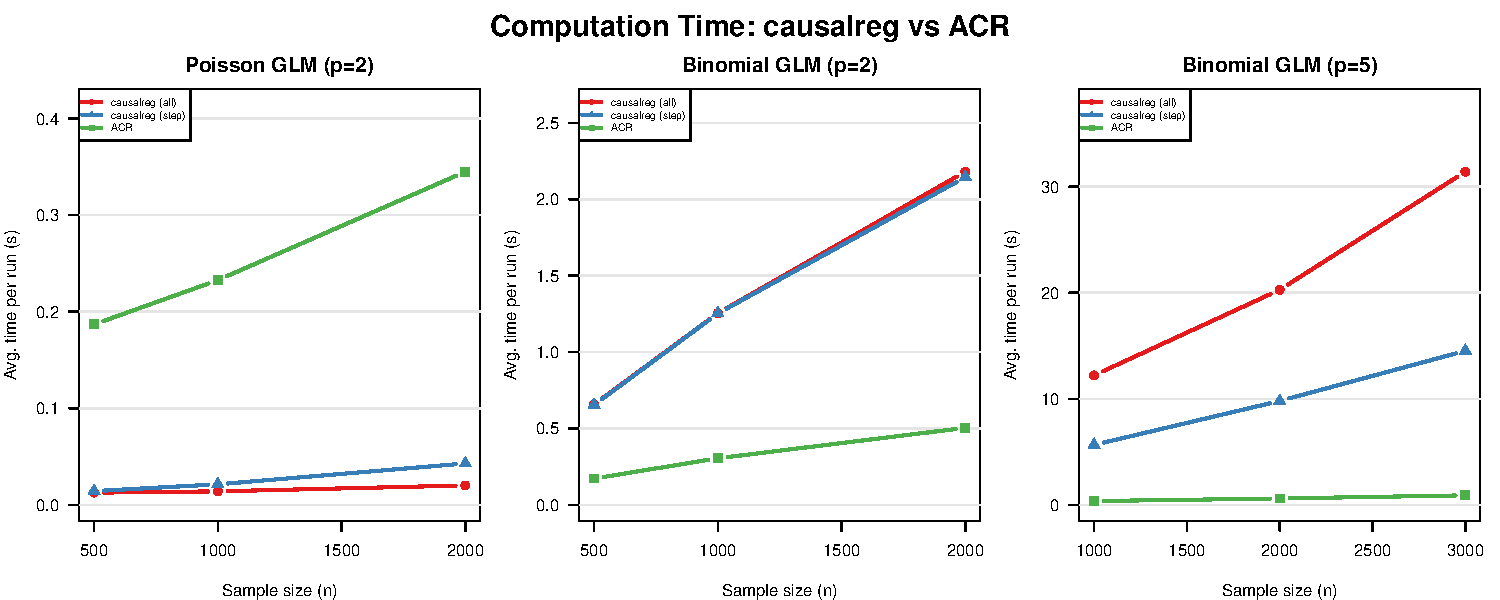
\includegraphics[width=\textwidth]{figures/fig_comparison_time.pdf}
\caption{Average computation time per run for \texttt{causalreg} and ACR.}
\label{fig:comparison_time}
\end{figure}

% ============================================================================
\section{Discussion}
% ============================================================================

\subsection{Pearson Risk Invariance (causalreg)}

The Pearson risk invariance method successfully recovers the true causal parents across a range of settings:

\begin{enumerate}
    \item \textbf{Sample size}: Recovery rates improve with increasing $n$ across all DGPs. For the simple two-covariate Poisson case (DGP~1), near-perfect recovery is achieved at $n = 500$. More complex scenarios (DGP~3 with $p=5$, DGP~5 with $p=7$) require larger samples.

    \item \textbf{Exhaustive vs.\ stepwise search}: The exhaustive search provides the best recovery guarantees, as it evaluates all possible subsets. The stepwise search is a practical alternative for larger $p$, with slightly lower recovery rates due to its greedy nature.

    \item \textbf{Chi-square vs.\ bootstrap}: For Poisson models, the chi-square test is fast and performs comparably to the bootstrap. For binomial models, the bootstrap is required, as the chi-square approximation does not hold.

    \item \textbf{Nonlinear models}: The GAM-based approach (DGPs~4--5) successfully handles nonlinear causal relationships by using smooth function terms, with recovery rates comparable to the linear case for similar problem complexity.

    \item \textbf{Robustness}: The method correctly distinguishes causal parents from ancestors ($X_1$ in DGP~3), descendants ($X_4$, $X_5$ in DGP~3), and spurious correlates, even in the presence of strong correlations.
\end{enumerate}

\subsection{Comparison with ACR}

The comparison reveals that the two methods have complementary strengths:

\begin{enumerate}
    \item \textbf{Model specification}: \texttt{causalreg} leverages the known response distribution (Poisson, binomial) through the Pearson risk, giving it a strong advantage on GLM data. ACR uses MSE loss regardless of the response type, which is suboptimal for discrete responses.

    \item \textbf{Environment discovery}: ACR's ability to discover latent environments can be valuable when distribution shifts are present but unlabeled. However, \texttt{causalreg} does not need environment information at all---it uses a model-based criterion that works with single-environment data.

    \item \textbf{Scalability}: ACR has fixed $O(n \cdot p^2 \cdot T)$ complexity where $T$ is the number of optimization steps, while \texttt{causalreg}'s exhaustive search has $O(2^p)$ complexity. For large $p$, ACR scales better; for small $p$ with discrete responses, \texttt{causalreg} is more appropriate.

    \item \textbf{Complementary use}: In practice, the methods address different settings. \texttt{causalreg} is the natural choice for count data (Poisson) or binary outcomes (binomial) with known distributional structure. ACR is better suited for continuous responses, high-dimensional settings, or when distribution shifts across environments provide additional causal signal.
\end{enumerate}

% ============================================================================
\section{Implementation Notes}
% ============================================================================

The \texttt{causalreg} package provides two main functions:

\begin{itemize}
    \item \texttt{cglm(formula, family, data, pval, search, ncores)}: causal discovery within a GLM.
    \item \texttt{cgam(formula, family, data, pval, search, ncores)}: causal discovery within a GAM.
\end{itemize}

Both support parallel computation via the \texttt{ncores} parameter, which distributes model evaluations across cores using \texttt{parallel::mclapply}. Typical speedups are 3--5$\times$ for exhaustive search on multi-core machines.

The package is available at \url{https://github.com/franciscorichter/causalreg}.

\bibliographystyle{plainnat}
\begin{thebibliography}{1}
\bibitem[Vinciotti and Wit(2026)]{vinciotti2026}
V.~Vinciotti and E.~C. Wit.
\newblock Causal generalized linear models.
\newblock \emph{causalreg: R package version 0.1.2}, 2026.
\newblock \url{https://CRAN.R-project.org/package=causalreg}.

\bibitem[Polinelli et~al.(2026)]{polinelli2026}
A.~Polinelli, V.~Vinciotti, and E.~C. Wit.
\newblock Causal generalized linear models via {P}earson risk invariance.
\newblock \emph{Journal of Causal Inference}, 2026.

\bibitem[Richter and Wit(2026)]{richter2026}
F.~Richter and E.~C. Wit.
\newblock Adversarial causal regularization without predefined environments.
\newblock Working paper, 2026.
\end{thebibliography}

\end{document}
